\documentclass[a4paper, 11pt, titlepage]{article}

\usepackage[utf8]{inputenc}
\usepackage{graphicx}
\usepackage{amssymb}
\usepackage{subfig}
\usepackage{amsmath}
\usepackage[pdfborder={0 0 0}]{hyperref}
\usepackage{fontspec}
\setmainfont[Mapping=tex-text]{Adobe Garamond Pro}

\begin{document}
\title{Crisis Response in Social Networks}
\author{Joseph F. Harrison \\
        Matthew Revelle \\
        CSS 692, Social Network Analysis \\
        George Mason University}
\date{May 2010}
\maketitle

\tableofcontents

\section{Introduction}

In \cite{Deards2009} ...

\begin{figure}[h]
\centering
\label{fig:all_tweets_over_time}
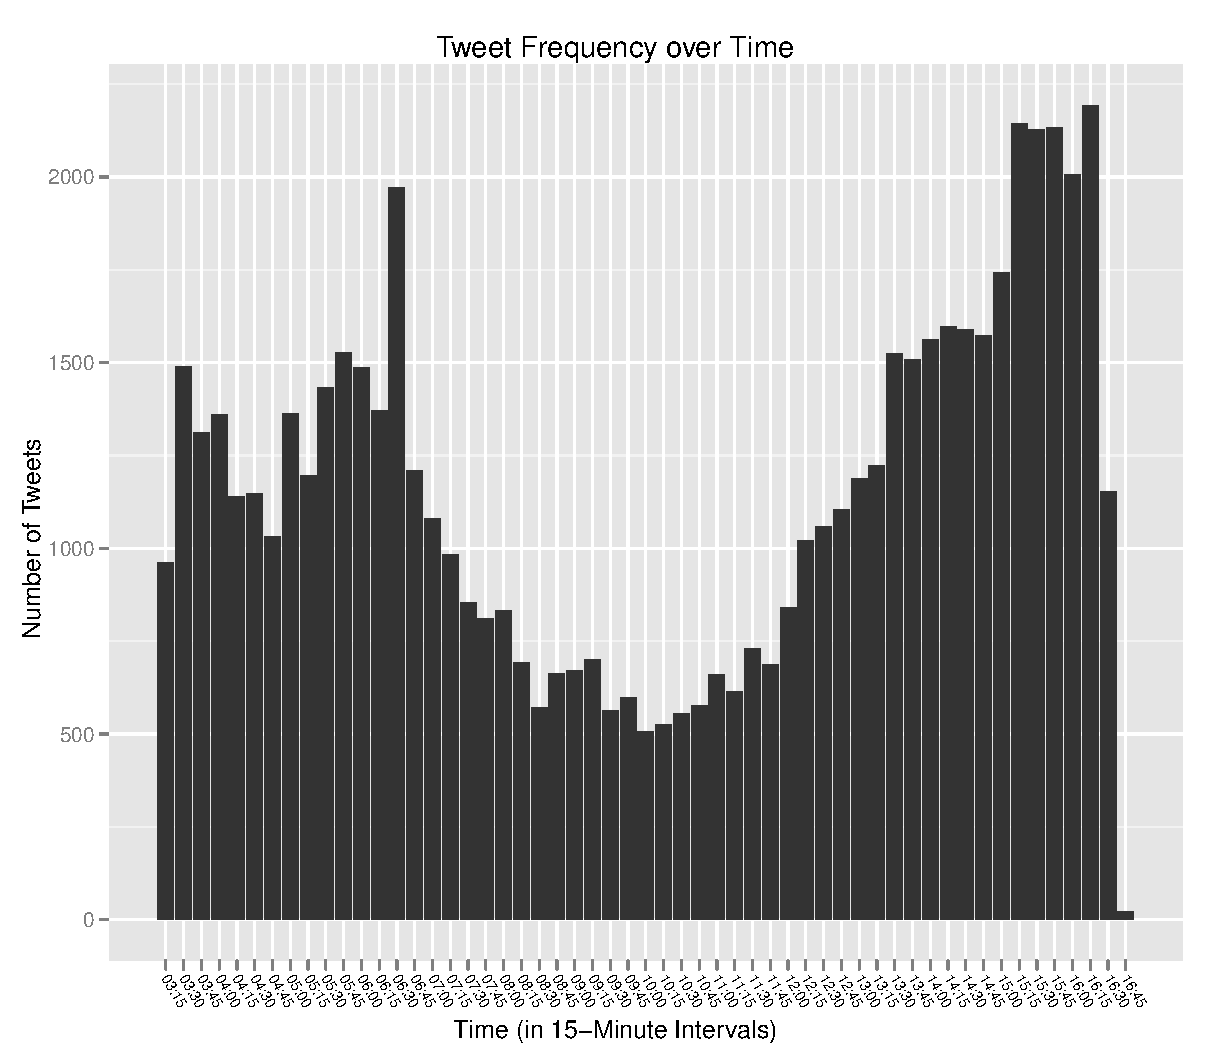
\includegraphics[width=120mm]{../figures/all_tweets_over_time}
\caption{All tweets over time..}
\end{figure}

\begin{figure}[h]
\centering
\label{fig:all_tweets_by_users}
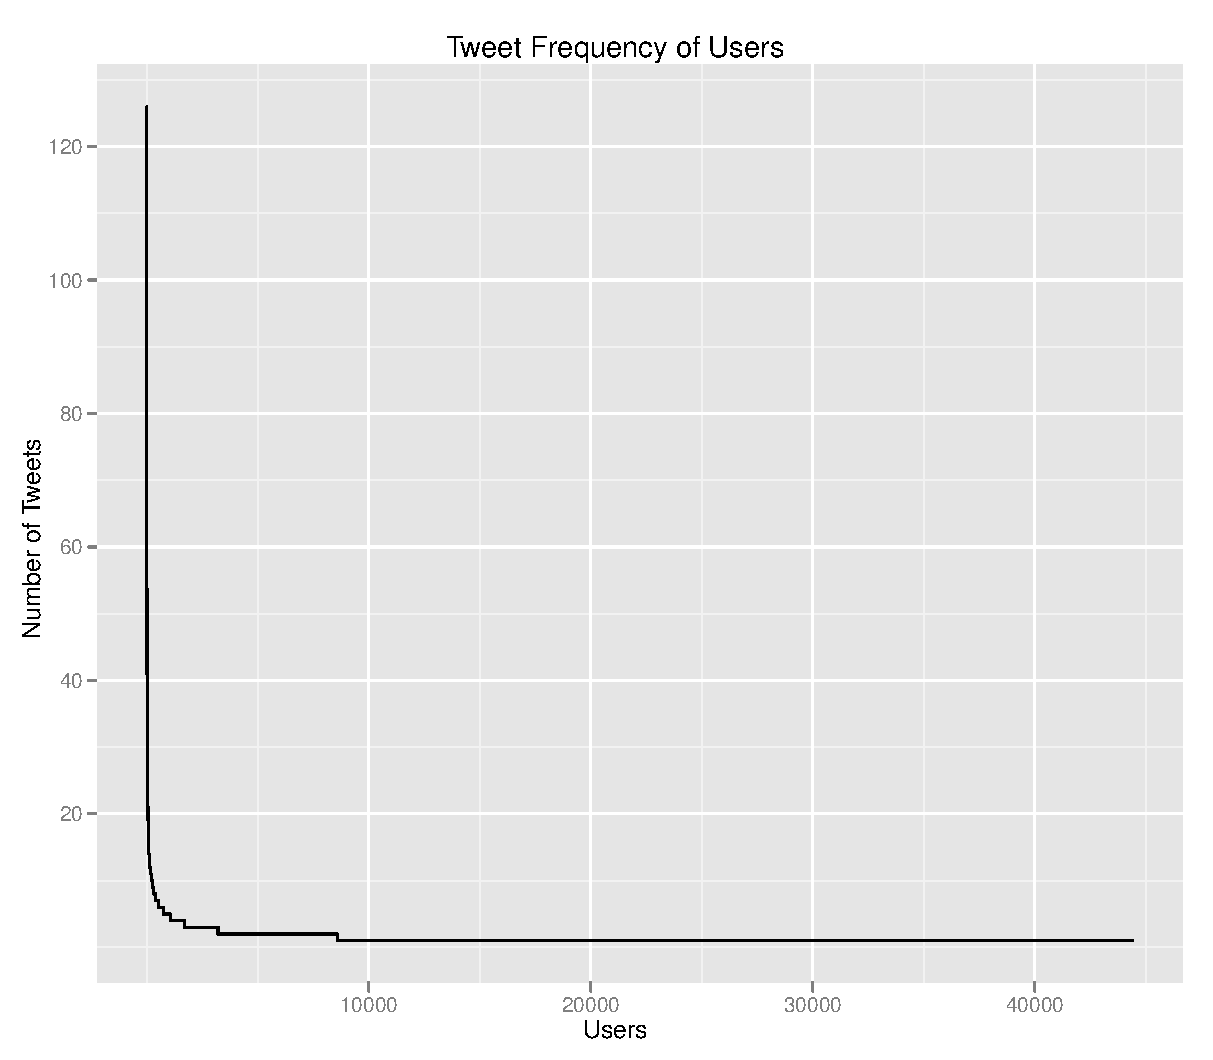
\includegraphics[width=120mm]{../figures/all_tweets_by_users}
\caption{All tweets over time..}
\end{figure}

\section{Retweets}

\begin{figure}[h]
\centering
\label{fig:rt_compare_over_time}
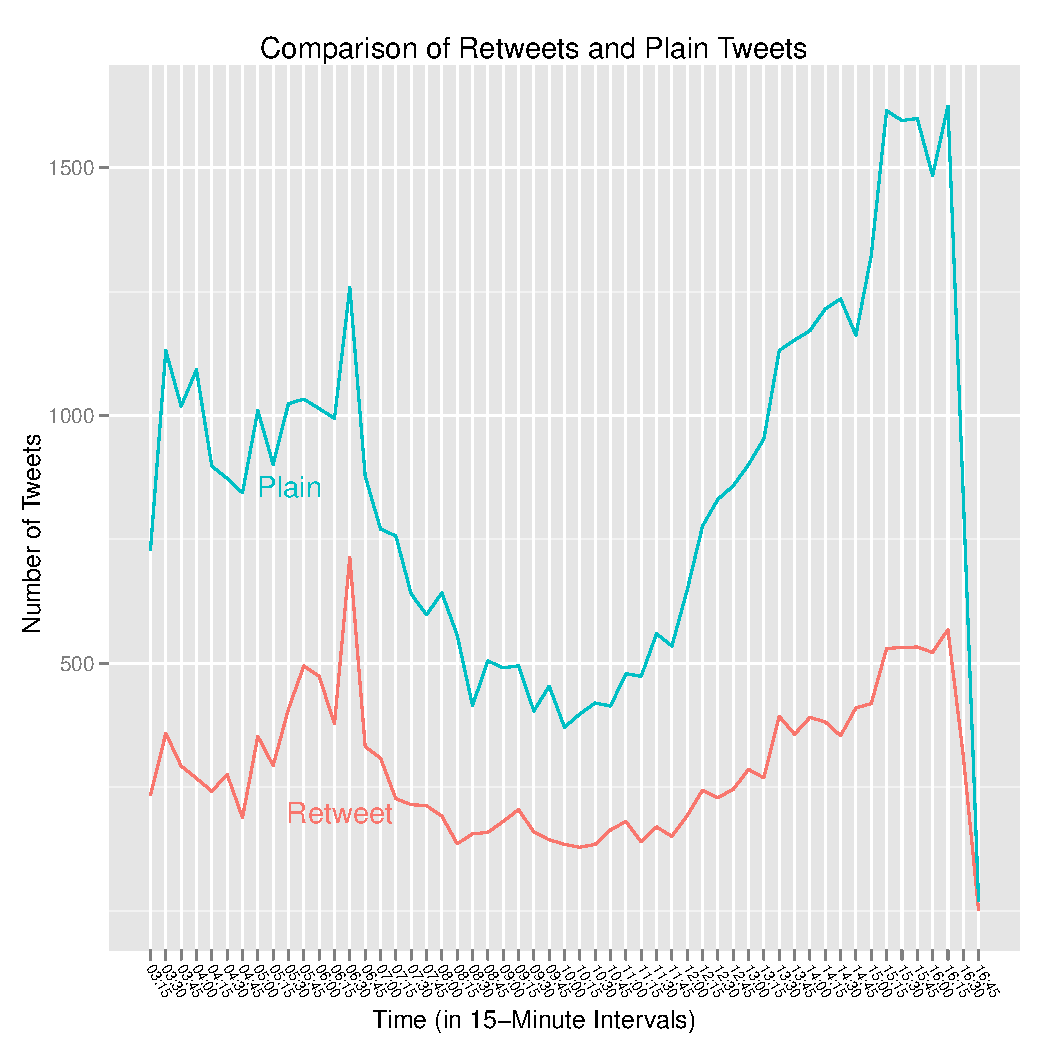
\includegraphics[width=120mm]{../figures/rt_compare_over_time}
\caption{Frequency of retweets compared to plain tweets over time.}
\end{figure}

\begin{figure}[h]
\centering
\label{fig:rt_top_50}
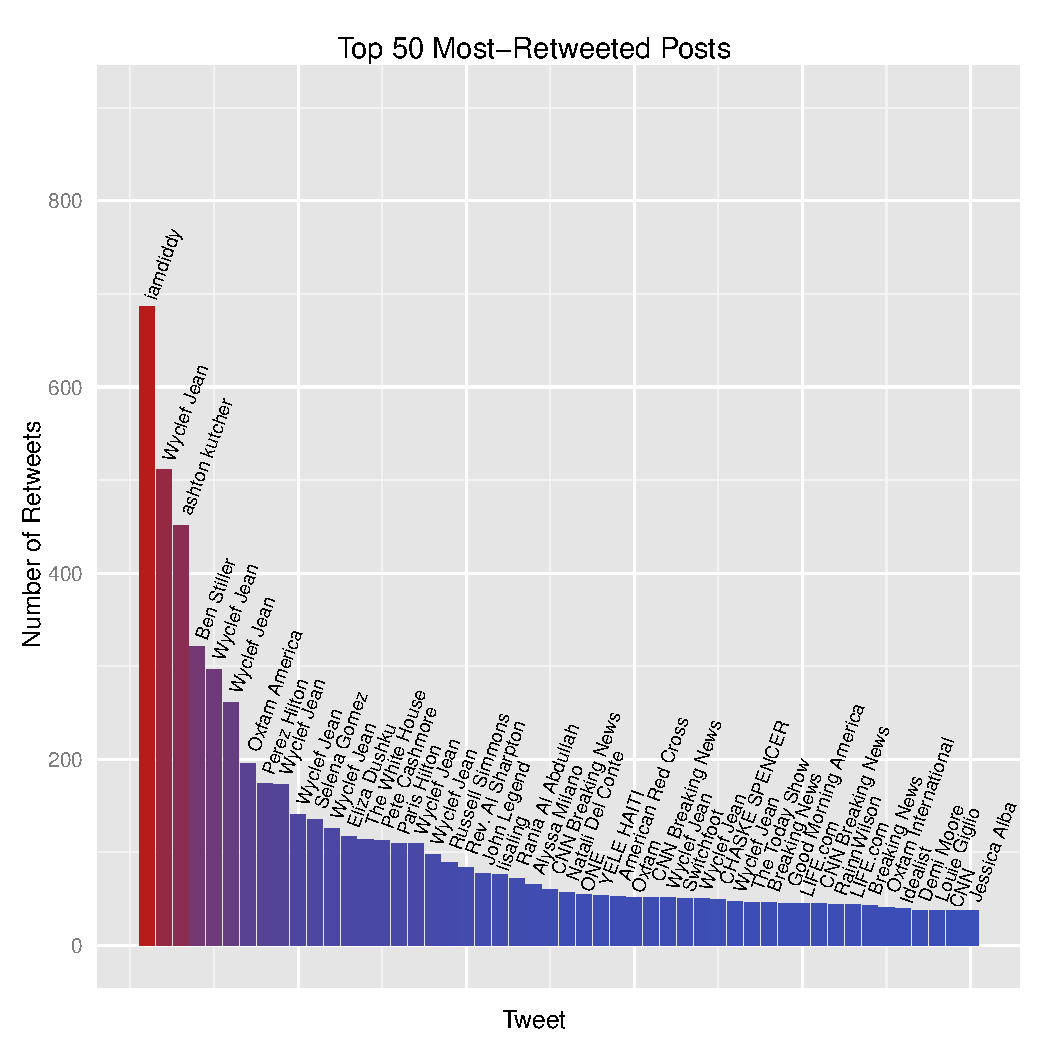
\includegraphics[width=120mm]{../figures/rt_top_50}
\caption{Top 50 most-retweeted posts.}
\end{figure}

\begin{figure}[h]
  \centering
\label{fig:rt_top_10}
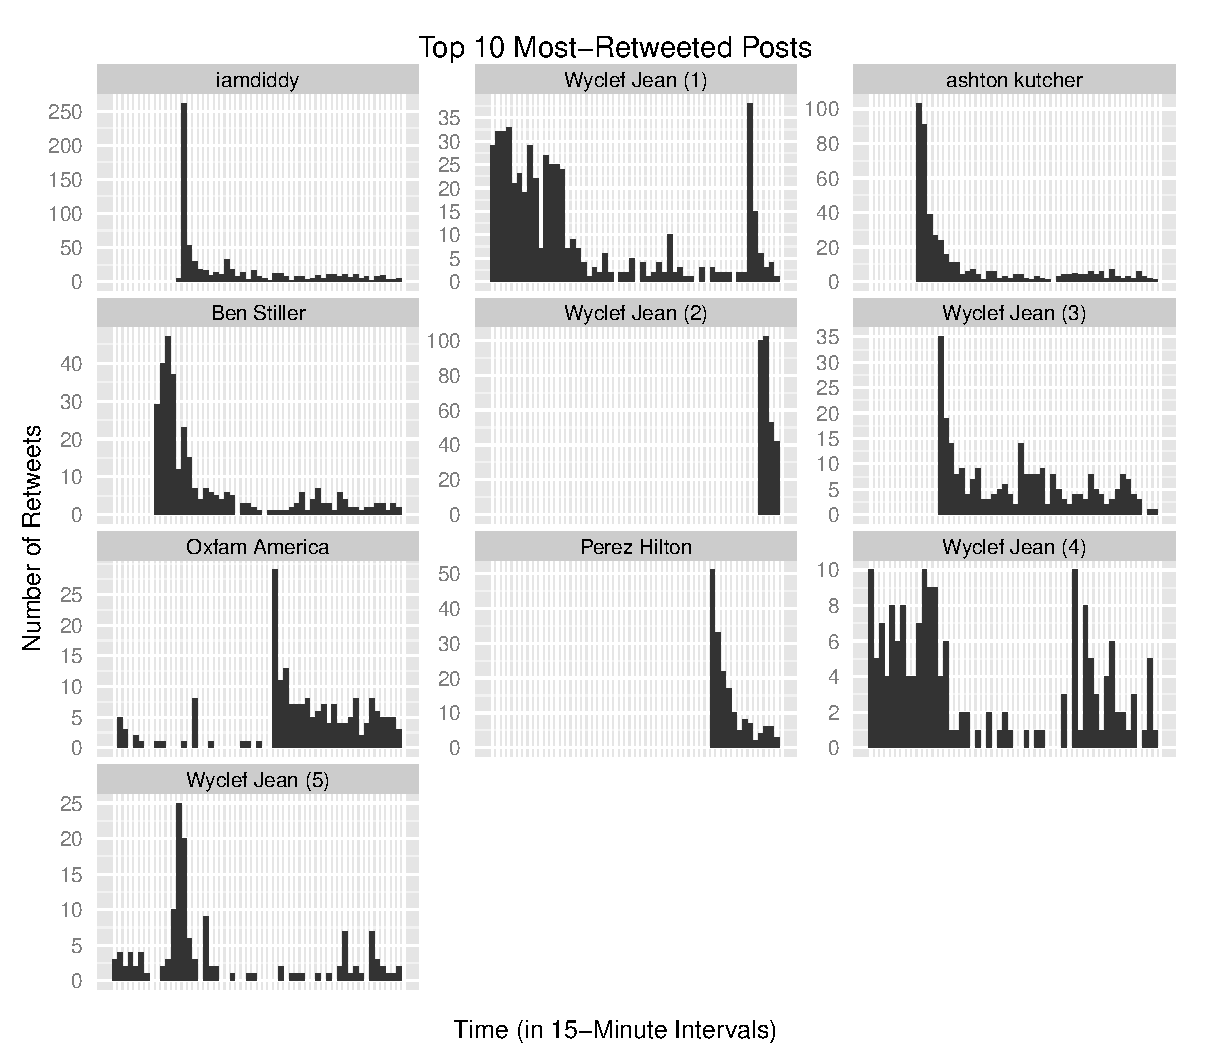
\includegraphics[width=120mm]{../figures/rt_top_10_over_time_free_scale}
\caption{Top 10 most-retweeted messages over time.}
\end{figure}

\begin{center}
  \begin{table}
    \caption{The author's name and message for the top 10 most-retweeted messages, sorted by number of retweets.}
  \begin{tabular}{| l | p{9.5cm} |}
    \hline
    \textit{Name} & \textit{Message} \\
    \hline
    iamdiddy & ``STATE OF EMERGENCY!!! RT PLEASE!!! Earthquake relief for Haiti please text YELE to 501501 to donate \$5 or go to www.yele.org RT PLS!!!'' \\
    \hline
    Wyclef Jean & ``Haiti is in need of immediate AID please text Yele to 510 510 and donate \$5 toward earthquake relief.'' \\
    \hline
    ashton kutcher & ``If you want to DONATE to HAITI EARTHQUAKE RELIEF: http://tinyurl.com/ya6kpzm'' \\
    \hline
    Ben Stiller & ``If you want to DONATE to HAITI EARTHQUAKE RELIEF: http://tinyurl.com/ya6kpzm'' \\
    \hline
    Wyclef Jean & ``Haiti needs your help text YELE to 501 501 and 5 dollars will go toward earthquake relief.'' \\
    \hline
    Wyclef Jean & ``Warriors Dontate to Earthquake relief in Haiti text Yele to  501 501 and visit www.yele.org'' \\
    \hline
    Oxfam America & ``Oxfam is already on the ground in \#Haiti after 7.0 magnitude earthquake hits. You can help now - please donate. http://bit.ly/8mrTkR'' \\
    \hline
    Perez Hilton & ``Another way you can help Haiti after their 7.0 earthquake: Donate \$5 by texting YELE to 501501 and by visiting www.yele.org'' \\
    \hline
    Wyclef Jean & ``Help Haiti Earthquake Relief Donate \$5 by texting YELE to 501 501 right now please RT'' \\
    \hline
    Wyclef Jean & ``Help Haiti Earthquake Relief Donate \$5 by texting YELE to 501 501 right now'' \\
    \hline
  \end{tabular}
  \end{table}
\end{center}

\begin{figure}[h]
\centering
\label{fig:rt_net_core}
\includegraphics[width=120mm]{../figures/rt_net_core}
\caption{The core of the retweet network.}
\end{figure}

\begin{figure}[h]
\centering
\label{fig:rt_net_top_50}
\includegraphics[width=120mm]{../figures/rt_net_top_50_tweets}
\caption{Top 50 most-retweeted posts in the network.}
\end{figure}

\begin{figure}[h]
\centering
\label{fig:rt_net_core_clusters}
\includegraphics[width=120mm]{../figures/rt_net_core_clusters}
\caption{Clusters in the network core.}
\end{figure}

\begin{figure}[h]
\centering
\label{fig:rt_net_travel}
\includegraphics[width=120mm]{../figures/rt_net_travel}
\caption{A cluster of tweets from authors in the travel industry.}
\end{figure}

\begin{figure}[h]
\centering
\label{fig:rt_net_photos}
\subfloat[Two Clusters]{\includegraphics[width=60mm]{../figures/rt_net_photo}}
\subfloat[Boundary Spanner]{\includegraphics[width=60mm]{../figures/rt_net_photo_popular}}
\caption{Clusters of tweets representing sets of photos.}
\end{figure}

\section{Groups}

\section{Conclusion}

\bibliographystyle{splncs}
\bibliography{bibfile}

\end{document}
